\paragraph{}
Durante todo el desarrollo del proyecto, han ido aparenciendo diversas dificultades y problemas que se debieron ir
resolviendo para el correcto y continuo avance del proyecto.

\paragraph{}
Por lo que en este capítulo se exlicarán las distintas soluciones, que se creian que podrían ser las mas acertadas,
encontradas a los principales problemas encontrados. 

%%%%%%%%%%%%%%%%% MOVIMIENTO COCHE %%%%%%%%%%%%%%%%%%%%
\section{Movimiento vehículo}


%%%%%%%%%%%%%%%%% CIRCUITOS %%%%%%%%%%%%%%%%%%%%%%%%%
\section{Formato y carga de circuitos}

\paragraph{}
Una de las primeras dudas que surgieron al poco tiempo de comenzar el desarrollo de \emph{Zycars}, fue el formato que deberían
tener los distintos circuitos o niveles que aparecerían a lo largo del juego. Para ellos tenía varias alternativas:

\begin{itemize}
    \item \textbf{Opción 1}: los circuitos estarían compuestos por una única imagen realizada posteriormente. En un fichero aparte se 
    podría indicar las zonas colisionables que tendría la imagen u otras características relevantes.
    
    \item \textbf{Opción 2}: crear los circuitos mediante un sistema de tieles, de formas que en un fichero de texto plano, indicáramos 
    los tieles que componen el circuito, así como la característica de estos.
    
    \item \textbf{Opción 3}: usar algún software que nos permitiera la creación y edición de niveles, de forma sencilla, mediante tiles.
\end{itemize}

\paragraph{}
Finalmente se optó por la opción 3, para ello se usó el programa \emph{Tiled} \footnote{Se comenta su uso y características en el
apéndice relacionado con las herramientas utilizadas}, dicho programa me proporcionaba todas las necesidades básicas, como una 
sencilla edición y creación de niveles, así como la gestión de capas, para poder poner elementos en el circuito a un nivel 
superior o inferior. Para ello se debia crear una imagen con todos los tiles que compondrían un circuito.

\paragraph{}
Este programa generaba como resultado un archivo \emph{XML}, que se procesaría posteriormente en tiempo de ejecución. También hay
que añadir que esta opción elegida era una de las que menos nos ocuparía en memoria, ya que no es lo mismo tener un circuito 
completo en una única imagen, ya que para un circuito demasiado grande dicha imagen ocuparía bastante memoria. Mientras
que con esta opción tendriamos una pequeña imagen con el conjunto necesario de tiles para el circuito en cuestión.

\paragraph{}
Una de las únicas cosas que no propocionaba el programa era poder indicar cuales de los tiles eran colisionables, atravesables o
de cualquier otro tipo. Así que para solventar este problema se elijió tener a parte de la imagen que contendría el conjunto de 
tiles otra imagen con las mismas características, como tamaño y el tamaño de los tiles, solo que esta ultima lo tiles tendrían 
colores planos indicando de que tipo serían. Así cuando cargaramos el circuito que necesitaramos en ese momento y con ello
el conjunto de tiles relacionado, se comprobaría que color tiene cada uno de los tiles en la otra imagen y así almacenar
de que tipo son. A continuación se muestran dos imagenes como ejemplo:

\begin{itemize}

    \item Este sería el aspecto de una imagen con el conjunto de tiles necesarios:
    \begin{figure}[H]
      \label{tileset}
      \begin{center}
        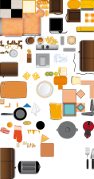
\includegraphics[scale=1]{imagenes/tileset.png}
      \end{center}
      \caption{Implementación: conjunto de tiles}
    \end{figure}
    
    \item Y esta la imagen que indicaría de que tipo son cada uno de los tiles de la imagen anterior:
    \begin{figure}[H]
      \label{collisionmap}
      \begin{center}
        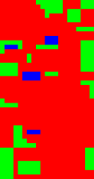
\includegraphics[scale=1]{imagenes/collisionmap.png}
      \end{center}
      \caption{Implementación: Mapa de colisiones}
    \end{figure}
    
\end{itemize}

\paragraph{}
Como se puede apreciar la imagen inferior tiene las mismas características que la superior, solo que los tiles que contiene
son de un único color para indicar el tipo de los tiles. Los tipos de tiles que se eligieron añadir fueron los siguientes:

\begin{itemize}
    \item \textbf{Rojo}: tiles completamentes atravesables, su única función es decorativa.
    
    \item \textbf{Verde}: tiles colisionables, aquellos que no pueden ser atravesados, normalmente marcan el recorrido
    del circuito, también usados como obstáculos.
    
    \item \textbf{Azul}: tiles atravesables, pero realentizan de forma considerable al vehículo que pase sobre ellos.
\end{itemize}

\section{Colisiones}

\paragraph{}
La detección de las colisiones es una de las cosas más básicas de la mayoría de los juegos en la que los jugadores
recorren mapas o niveles.

\paragraph{}
En \emph{Zycars} debemos de gestionar varios tipos de colisiones, entre esos tipos estaría la colisión que se produciría 
entre cualquier vehículo y el escenario en el que se encuentre, así como la colisión entres dos objetos del juego, como podrían
ser desde dos vehículos entre si, o algún vehículo por algun item lanzado por otro jugador.

\paragraph{}
Indicar que cada uno de los objetos que intervienen en el juego y puede colisionar con cualquier elemento, tienen
un rectangulo asociado a su forma, de manera que sea mas sencilla la detección de colisiones.

\paragraph{}
En las siguiente subsecciones se explicará cuales son las soluciones que se llevaron a cabo para la gestión de las colisiones 
en cada una de las situaciones posibles.

\subsection{Colisión con el escenario}

\paragraph{}
Como se comento en el apartado dedicado a la carga y formato de los circuitos, cada uno de los circuitos tiene asociado una imagen
que indica de que tipo es cada uno de los tiles que nos podemos encontrar a lo largo del circuito.

\paragraph{}
Así que a la hora de cargar el circuito en el que vayamos a competir almacenabamos cada uno de los tiles que componían el circuito,
así como el tipo que eran. Dada esta situación debemos ir comprobando si el jugador esta atravensando algún tile colisionable. 
Si es el caso debemos corregir la posición del objeto con respecto al tile con el que estaba colisionando.

\paragraph{}
A la hora de realizar la correción de la colisión, debemos tener en cuenta aspectos como, ángulo del vehículo, dirección del 
vehículo, así como el lado del tile por el que se produce la colisión, ya sea por la parte superior, inferior o alguno 
de los laterales. Según estos parámetros la collisión se corregirá en una dirección u otra.

\paragraph{}
A continuación se expone un ejemplo visual para su correcta comprensión:

\begin{itemize}
    \item Se detecta que un vehículo colisiona con un tile colisionable:
    \begin{figure}[H]
      \label{colision1}
      \begin{center}
        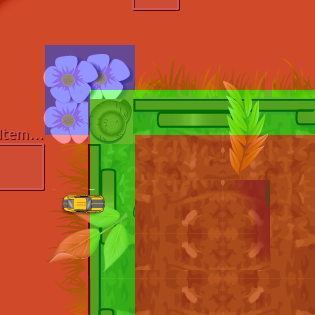
\includegraphics[scale=0.4]{imagenes/colision1.png}
      \end{center}
      \caption{Implementación: Colisión con el escenario 1/2}
    \end{figure}
    
    \item Se corrige la colisión en función del ángulo y dirección del vehículo, asi como el lado por el que colisiona del tile:
    \begin{figure}[H]
      \label{colision2}
      \begin{center}
        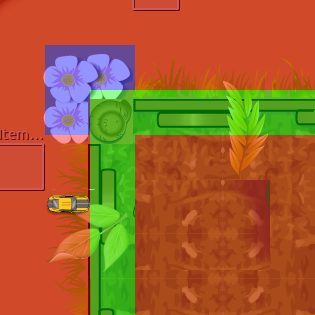
\includegraphics[scale=0.4]{imagenes/colision2.png}
      \end{center}
      \caption{Implementación: Colisión con el escenario 2/2}
    \end{figure}
    
\end{itemize}

\paragraph{}
En el caso de que se colisione con un tile que atravesable pero era del tipo que realentizaban la velocidad, únicamente
se reducirá la velocidad del vehículo y no se corregira su posición para este tile.


\subsection{Colisiones entre objetos}

\paragraph{}
En este caso hay varias posibilidades según que tipos de objetos han colisionado, en todas ellas la detección de la colisión
se hace de forma similar, comprobamos si alguna de las caja de colisiones de los objetos en cuestión se superponen o no.

\paragraph{}
A continuación se exponen las distintas situaciones que pueden suceder:

\begin{itemize}
    \item \textbf{Colisión vehículo-vehículo}: dos vehículos en carrera colisionan entre sí, en este caso debemos comprobar 
    cual de los dos vehículos ha colisionado con el otro, es decir, cual se ha interpuesto. En ese caso 
    corregiremos la posición de ese vehículo y produciremos algún tipo de rebote en función de la velocidad que llevara
    en ese momento.
    
    \item \textbf{Colisión vehículo-item}: en este caso se responderá a la colision dependiendo del tipo de item con el que
    hemos colisionado.
    \begin{itemize}
        \item Si el item es un misil o una bola, el item pasará a su estado de explosión, mientras que el vehículo parasa a un estado de daño
        
        \item Si el item es una mancha de aceite, el item no cambiará su estado, pero el coche pasar a un estado de descontrol durante
        unos instantes
        
        \item Si el item es un chicle, se reducirá de forma considerable la velocidad del vehículo.
    \end{itemize}
\end{itemize}

%%%%%%%%%%%%%%%%%%%% INTELIGENCIA ARTIFICIAL %%%%%%%%%%%%%%%%%%%%%%%%
\section{Inteligencia artificial}

\subsection{Realización del recorrido. A*}

\subsection{Lanzamiento de items.}
